\documentclass[11pt]{article}
\usepackage[margin=0.9in]{geometry}
\usepackage{booktabs,amsmath,amssymb,array,xcolor,enumitem,tikz}
\usepackage[colorlinks=true,linkcolor=blue!50!black,urlcolor=blue!50!black]{hyperref}
\setlist{itemsep=2pt,topsep=3pt}
\newcommand{\say}[1]{\begin{quote}\itshape #1\end{quote}}
\definecolor{box}{HTML}{EEF3FA}
\newcommand{\keybox}[1]{\par\noindent\colorbox{box}{\parbox{\dimexpr\linewidth-2\fboxsep}{#1}}\par\medskip}

\title{Presentation Guide\\\large Resequencing Blame: an airport-game theory of cross-flow head-of-line blocking}
\author{Adhyan Jain \and Atharva Sheersh Pandey \and Kshitij Manikshete}
\date{}
\begin{document}
\maketitle

\section{The 30-second version}
\keybox{\textbf{Problem.} In Wi-Fi~7 multi-link operation, packets of different flows share one reorder buffer. A slow link can make a latency-sensitive flow wait for \emph{another} flow's late packet. Everyone measures this wait; nobody could say \emph{which other flow} is responsible, or by how much, without re-running the whole simulation many times.\\[3pt]
\textbf{Our finding.} The wait a packet suffers because of other flows equals the \emph{largest lateness among them}. That is exactly the \textbf{airport game}: a runway is as long as the biggest plane needs, and the cost is shared fairly among planes. Its fair split (the Shapley value) has a closed form, so blame can be computed \emph{exactly from one recorded trace}, with no re-runs.\\[3pt]
\textbf{Why it holds up.} It is proved, it survives real receiver behaviour (finite window, timeouts), and it was checked exactly on our simulator, on stress traces, and on ns-3's own reorder buffer.}

\section{Explain it in four steps (the core of the talk)}
\subsection*{Step 1: what a reorder buffer does}
\say{The receiver hands packets up in sequence-number order. If packet 7 hasn't arrived, packets 8, 9, 10 wait, even if they belong to a different flow. That waiting is head-of-line blocking.}

\subsection*{Step 2: the key observation}
\say{A packet is released at the moment it and \emph{all earlier packets} have arrived. So its release time is a running maximum of arrival times. The part of the wait caused by other flows is therefore the \emph{maximum} over the other flows of how late each one is, not the sum.}
Define \emph{lateness} of flow $j$ for a victim packet: how long after the victim's own flow is complete the latest earlier packet of flow $j$ arrives. Then
\[
\text{cross-flow blocking}=\max_j \ell_j .
\]
A maximum of lateness values is exactly the airport-game cost function.

\subsection*{Step 3: the example to draw on the board}
\begin{center}
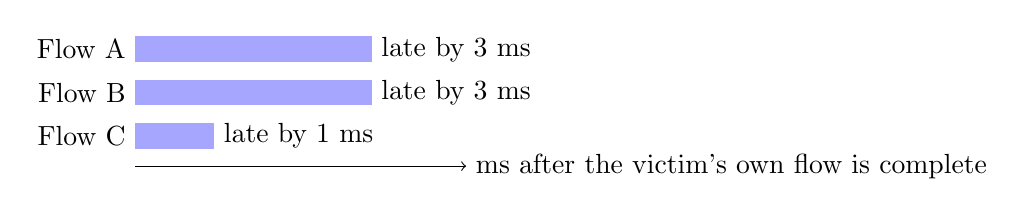
\begin{tikzpicture}[x=1.0cm,y=0.55cm]
\foreach \y/\w/\n in {3/3/Flow A,2/3/Flow B,1/1/Flow C}{
  \fill[blue!35] (0,\y) rectangle (\w,\y+0.6); \node[left] at (0,\y+0.3) {\n}; \node[right] at (\w,\y+0.3) {late by \w\ ms};}
\draw[->] (0,0.6) -- (4.2,0.6) node[right] {ms after the victim's own flow is complete};
\end{tikzpicture}
\end{center}
The victim waits 3 ms in total (two flows are equally the latest). Who is to blame?
\begin{center}
\begin{tabular}{lccc}
\toprule
Rule & Flow A & Flow B & Flow C\\
\midrule
Leave-one-out (remove a flow, see what changes) & 0 & 0 & 0\\
``Last arrival takes all'' (what a trace tool reports) & 3 & 0 & 0 \emph{or} 0, 3, 0\\
\textbf{Shapley (ours)} & \textbf{4/3} & \textbf{4/3} & \textbf{1/3}\\
\bottomrule
\end{tabular}
\end{center}
\say{Leave-one-out explains none of the 3~ms, because removing either tied flow changes nothing. The usual rule blames one flow arbitrarily. Shapley splits it fairly: the first millisecond among all three flows (they were all late at least that long), the remaining two among the two that were later.}

\subsection*{Step 4: what you get from it}
\begin{enumerate}
\item \textbf{Exact blame from one trace}, in $O(m\log m)$ per packet, instead of $2^m$ counterfactual runs (22$\times$ faster already with 3 other flows).
\item \textbf{Why the alternatives fail}, proved: leave-one-out misses exactly the second-largest lateness; ``last arrival'' can flip arbitrarily under a tiny timing change.
\item \textbf{Worst-case stability}: Shapley blame changes by at most 2$\times$ the change in lateness, whatever the load, number of flows, or window.
\item \textbf{Real receivers}: with a finite window and a hold timer the same law holds once arrival times are replaced by the time each slot is \emph{resolved}; the gap to the ideal case is bounded by $2m\delta$, and a per-packet certificate says where the theory applies.
\end{enumerate}

\section{What is new and what is not (say this honestly)}
\begin{center}
\begin{tabular}{p{0.30\linewidth}p{0.62\linewidth}}
\toprule
Not ours (classical) & Resequencing delay analysis (Baccelli--Gelenbe--Plateau 1984; Han--Makowski 2005); the airport game and its Shapley value (Littlechild--Owen 1973; Dubey 1982); Shapley in queueing and networking (Maniquet 2003; Ma et al.\ 2010).\\
\textbf{Ours} & Recognising that cross-flow reordering blame \emph{is} an airport game, and everything that follows: closed form without replay, exact degeneracy of leave-one-out and last-arrival, stability constant 2, extension to windows and timers with a bound and certificate, and independent confirmation on ns-3's reorder buffer.\\
Caveat to state yourself & The core proof is short. The value is the identification plus its consequences plus unusually strong verification. Our literature search was limited, so say ``to our knowledge''.\\
\bottomrule
\end{tabular}
\end{center}

\section{Evidence in one table (what, where, how strong)}
\begin{center}\small
\begin{tabular}{p{0.26\linewidth}p{0.36\linewidth}p{0.28\linewidth}}
\toprule
Claim & Evidence & Where\\
\midrule
Blocking = max lateness (airport game) & Real receiver re-run on traces with flows deleted; 700 simulator runs, error $\le 2.3\times10^{-13}$ & Study 5; \texttt{results/analysis\_study5.json}\\
Forced release (window, timer, loss) & 900 traces, 18 configurations, 249{,}142 packets, 16{,}554 forced events, error 0, 0 set mismatches & Study 6; \texttt{analysis\_study6.json}\\
Independent implementation & ns-3.47's own buffer: 3{,}253{,}034 packets, release-law error exactly 0 & Study 6 (H22--H24)\\
Queueing is super-additive & Non-additivity of queueing part $1.89$ and $1.74$, intervals above 1 & Study 5 (H17)\\
Worst-case stability & Max change ratio 1.00 (Shapley, bound 2) vs 348 (last-arrival rule) & Study 5 (X13)\\
Explained-fraction bound $r\ge q$ & 0 violations in 13 Python + 6 ns-3 held-out cells; rank correlation 0.93 & Study 4\\
\bottomrule
\end{tabular}
\end{center}
\noindent Every number in the manuscript is generated from stored result files (\texttt{make\_numbers*.py}); each study was preregistered, hashed and committed before its data.

\section{Limits and failures: say them before they are asked}
\begin{itemize}
\item \textbf{Simulation only}: no hardware, no public external trace.
\item \textbf{Rules rarely differ in practice here}: in the simulator and in ns-3 most blocked packets have a single late flow, so all three blame rules agree. The rules differ when several flows are late (our generators; high-load ns-3 cells: 2--16\% of blocked packets).
\item \textbf{No decision benefit shown}: choosing which flow to remove by Shapley was not better than by trace blame.
\item \textbf{Shapley is more stable only in the worst case}, not on average (a preregistered test failed).
\item \textbf{Certificate is conservative}: 44\% of delivered packets certified in the stress traces.
\item \textbf{Not tested}: ns-3's own block-ack-request forced release, duplicates, real hardware. The timer receiver is our own implementation.
\item \textbf{Other preregistered failures}, all reported: Study 2 validity control, Study 3 exact check (one row) and a flawed decision metric, a numerical-convergence criterion in the Poisson baseline.
\end{itemize}

\section{Talk structures}
\subsection*{5 minutes (viva or quick pitch)}
\begin{enumerate}
\item (0:45) Problem: shared reorder buffer, who is to blame.
\item (1:30) Key observation and the 3-flow example (draw the bars and the table).
\item (1:00) Consequences: exact, replay-free, why leave-one-out fails, stability.
\item (1:00) Evidence: one headline number each (700 runs, 900 traces, 3.25M ns-3 packets).
\item (0:45) Honest limits, then ``what we would do next''.
\end{enumerate}
\subsection*{15 minutes (department talk)}
Add: model and release law (2 min); the Shapley closed-form derivation via the staircase $\ell_{(s)}-\ell_{(s-1)}$ (3 min); forced release and the certificate (3 min); the preregistration discipline and the failures (2 min).

\section{Live demo (2 minutes, optional)}
\begin{verbatim}
cd validation/pairing
../../.venv/bin/python -m pytest -q tests             # 131 tests pass
../../.venv/bin/python analyze_study6.py              # recompute headline results from raw CSVs
../../.venv/bin/python -c "import airport as a; \
print(a.shapley_airport([3,3,1]))"
# -> [1.3333 1.3333 0.3333]
\end{verbatim}
Open \texttt{README.md} (map of everything), then \texttt{paper/theory/main\_theory.pdf}, then \texttt{AUDIT\_REPORT.md} to show the integrity checks.

\section{Likely questions and short answers}
\begin{description}[leftmargin=0pt,style=nextline]
\item[``Isn't this just Shapley applied to delay?''] No: the contribution is showing the blocking game has airport structure, which is what makes the closed form, the exact failure of leave-one-out, and the stability bound possible. Shapley on arbitrary delay games needs exponential replays.
\item[``Is the proof trivial?''] The core is short, and we say so. The work is in the consequences and in verifying them exactly, including on third-party code.
\item[``Real receivers drop and time out.''] Handled: with a finite window and hold timer the law holds on resolution times, the gap to ideal blame is bounded, and a certificate flags packets where it does not apply. Not covered: ns-3's block-ack-request release, hardware.
\item[``Your simulator, your results.''] Partly answered: the release law holds exactly in ns-3.47's own reorder buffer (3.25M packets) and our receiver reproduces its release times. The traffic scenarios are ours.
\item[``Does it improve anything?''] We do not claim it does; the value is an exact, cheap attribution with guarantees. A decision test found no benefit.
\item[``Why Shapley and not something else?''] On airport games it is the unique rule satisfying the standard axioms (Dubey 1982), and the competing trace rules are provably degenerate. We did not compare nucleolus or serial rules.
\item[``Why should I trust the numbers?''] Six preregistered studies, hashes and commit order audited, analyses reproduce byte for byte, headline numbers recomputed independently (\texttt{AUDIT\_REPORT.md}).
\end{description}

\section{Where everything is}
\begin{center}\small
\begin{tabular}{p{0.38\linewidth}p{0.54\linewidth}}
\toprule
File & Use it for\\
\midrule
\texttt{README.md} & Map of the project and reproduce commands\\
\texttt{paper/theory/main\_theory.pdf} & Main manuscript: theorems, proofs, validation\\
\texttt{paper/main.pdf} & Companion paper: counterfactual externality and the explained-fraction bound\\
\texttt{NOVELTY\_SUMMARY.md} & One-page novelty and limits\\
\texttt{AUDIT\_REPORT.md} & Integrity checks and remaining gaps\\
\texttt{decisions.md} & Why each major decision was made (D01--D33)\\
\texttt{airport.py}, \texttt{study6.py} & The blame formula, oracles, window/timer receiver\\
\texttt{PREREGISTRATION\_STUDY*.md} & What was predicted before each study ran\\
\bottomrule
\end{tabular}
\end{center}

\section{Glossary}
\begin{description}[leftmargin=0pt,style=nextline]
\item[Reorder buffer] Receiver memory that holds out-of-order packets until earlier sequence numbers arrive.
\item[Cross-flow blocking] The wait of a packet caused by other flows' late packets.
\item[Lateness $\ell_j$] How long after the victim's own flow is complete the latest earlier packet of flow $j$ arrives.
\item[Airport game] Cost-sharing game where a coalition costs as much as its largest member.
\item[Shapley value] The fair split averaging each player's marginal contribution over all orderings.
\item[Leave-one-out] Blame = change when one flow is removed.
\item[Effective arrival] The time a sequence slot is resolved, by its own packet or by a forced advance (window or timer).
\item[Certificate] A per-packet check, from recorded events only, of whether the exact theory applies.
\item[Preregistration] Hypotheses and thresholds written, hashed and committed before the data exist.
\end{description}
\end{document}
